\section{Applicability to Other LSH Indices}
\label{sec:extension}

We discuss the possibilities of applying our approach to other LSH variants in this section.

%As long as the basic index structure is a hash table or B-tree, it is possible to rebuild the index with multi-layered structure by leveraging density of hash values.
\subsection{Table-based LSH and LayerDSH}
\label{sec:extension:dsh}

The idea of rehashing points with multi-layered structure should work as long as the basic index structure is a hash table.
%The data points in heavy loaded buckets can be reorganized to achieve better performance.
For example, \textbf{C2LSH} \cite{c2lsh} randomly chooses a number of LSH functions to form a function base and performs $k$NN query based on the intuition that a query $q$ should collide with its close neighbors under a large number of LSH functions. Though the idea is novel, the basic indexing structure is a hash table, so that we can reorganized the points in dense buckets using the multi-layered structure to improve efficiency. In addition, \textbf{DSH} \cite{Gao:2014:DDS:2588555.2588565} and \textbf{Selective Hashing} \cite{Gao:2015:SHC:2783258.2783284} were recently proposed to address the unbalanced data distribution problem, which can also integrate the multi-layered structure to further balance the hash table. We briefly demonstrate the idea of rebuilding DSH as follows.

%However, how to guarantee the search quality after integrating multi-layered structure is an open problem for these LSH variants.

\Paragraph{LayerDSH} DSH \cite{Gao:2014:DDS:2588555.2588565} aims to build data-sensitive hash family for the skewed data and directly answers $k$NN query. The DSH family is defined as follows \cite{Gao:2014:DDS:2588555.2588565}:
\begin{definition}
\label{def:dsh}
(\textbf{DSH family}) A family $\mathcal{H}=\{h:R^d\rightarrow\{0,1\}\}$ is called $(k,ck,p_1,p_2)$-sensitive if for any query point $q\in R^d$ and $o\in O$
\begin{itemize}
  \item If $o\in NN(q,k)$ then $\frac{|\{h|h(o)=h(q),h\in\mathcal{H}\}|}{|\mathcal{H}|}\geq p_1$,
  \item If $o\notin NN(q,ck)$ then $\frac{|\{h|h(o)=h(q),h\in\mathcal{H}\}|}{|\mathcal{H}|}\leq p_2$.
\end{itemize}
\end{definition}
The DSH family can be learned from the data and generated by combining adaptive boosting and spectral techniques \cite{Gao:2014:DDS:2588555.2588565}, which is endowed with good theoretical guarantee.

Even though the points are distributed more evenly and the buckets are more balanced in DSH than that in LSH, the buckets are not totally balanced as shown in the experimental results \cite{Gao:2014:DDS:2588555.2588565}. As DSH aims to generate proper hash families to generate balanced hash tables, our idea can be applied to the DSH tables as a postprocessing step to further balance the hash tables. We propose LayerDSH which rehashes the dense buckets and merges the sparse buckets for DSH. The building process of LayerDSH is similar to LayerLSH. According to the definition of DSH, the expected recall $\alpha$ should be set as $\alpha=p_1$ which is defined in Definition \ref{def:dsh}. In addition, to sustain the success probability, the probability $p$ appeared in Proposition \ref{prop:accuracy} and \ref{prop:efficiency} should be set as $p=p_1$ instead of $p=p(r^*,w)$.


\subsection{Tree-based LSH and LayerLSB}

There exist several tree-based LSH index structures, such as LSB \cite{lsb}, LSH Forest \cite{Bawa:2005:LFS:1060745.1060840}, and SK-LSH \cite{sklsh}. \textbf{LSH Forest} \cite{Bawa:2005:LFS:1060745.1060840} exploits tree structure to manage hash values. Each hash function applied on an object produces one bit. Each object is assigned with a label containing a sequence of bits that are generated from multiple hash functions, such that the close points are assigned with similar labels. Since the sequence of bits can be linearly ordered, they are indexed by a tree. A collection of multiple LSH trees forms a \emph{LSH Forest}. \textbf{SK-LSH} \cite{sklsh} defines a new distance measure of two hash values which captures the similarity of two points, so that the hash values can be linearly ordered and indexed by B-tree structure. By exploring the density of hash values, both of the two tree-based LSH indices can be rebuilt with multi-layered structure.


\Paragraph{LayerLSB}
The \textbf{LSB} approach constructs an LSB-tree structure and performs approximate NN queries by exploiting the tree structure \cite{lsb}. Each multi-dimensional object $o$ is reduced to a one-dimensional $z$-value $z(o)$ \cite{Gaede:1998:MAM:280277.280279}. The multi-dimensional objects can be organized in the numerical order of their $z$-values and are indexed by a conventional B-tree. The close points in high dimensional space exhibit similar $z$-values, so that the $k$NN search for a query $q$ is translated into one dimensional range search on the $z$-values around query $q$'s $z$-value. This is the basic idea of LSB-tree. In addition, multiple LSB-trees can be built to improve search quality. The approximate $k$NN query is achieved by a synchronous bi-directional expansion at the leaf levels of all LSB-trees.

\begin{figure}[t]
\vspace{-0.1in}
    \centerline{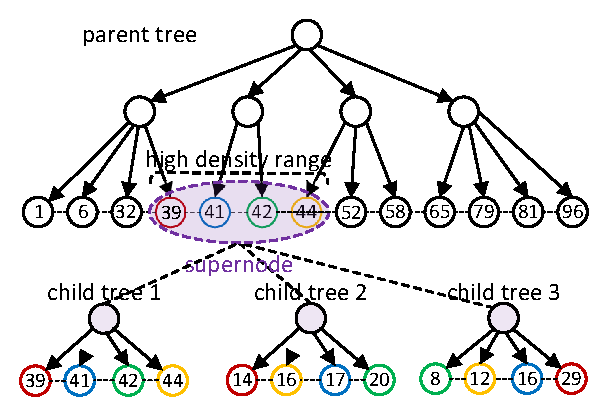
\includegraphics[width=2.6in]{fig/layerlsb.eps}}
    \caption{An illustrative example of LayerLSB structure. The circles with the same color indicate the same original data point. The number inside each circle is the $z$-value of that point in a particular LSB-tree.}
    \label{fig:layerlsb}
\end{figure}

We propose LayerLSB structure by exploring the density of $z$-values. Since the queries falling in high density ranges usually exhibit low search quality, extra efforts are put into building indices for these queries. Figure \ref{fig:layerlsb} shows an illustrative example of LayerLSB structure. The leaf nodes in high density ranges are rehashed in multiple independent child LSB-trees. These leaf nodes in parent tree are merged as a \emph{supernode}. The original $z$-values obtained in parent LSB-tree are retained in the first child tree. Two extra child trees with a new set of LSB parameters are further created. As a result, new $z$-values of these rehashed data points are obtained.

Even though only two levels are shown in Figure \ref{fig:layerlsb}, it is possible to further rehash the level-1 child LSB leaf nodes and create level-2 child LSB-trees. This results in a \emph{multi-layered} LSB-trees structure. This variation of $z$-values' order achieved by extra LSHs will increase the probability of returning the real $k$NNs. Comparing to blindly creating more LSB-trees without discrimination, great efforts can be saved by targeted rehashing. A small number of root level LayerLSB-trees is enough to achieve high search quality.
